\paragraph{Мейн информация}
Программа task\_7 является ELF исполняемым файлом.
Это текстовый энкодер, принимающий строку текста в качестве аргумента.

\paragraph{Описание}

\begin{itemize}
    \item Если программа запускается корректно, выполнение продолжается.
    \item Если программа запускается некорректно, выводится сообщение: "Usage: ./task\_7 TEXT"
    \item Программа выделяет память для локальных переменных.
    \item Для каждого символа входной строки выполняется последовательность операций:
    \begin{itemize}
        \item К символу добавляется его позиция в строке (ADD)
        \item Выполняется операция XOR с числом 14 (0xE)
        \item Применяется маска через AND с числом 31 (0x1F)
        \item Из результата вычитается (позиция + 1)
    \end{itemize}
    \item Результат выводится в консоль в виде бинарных данных.
\end{itemize}

\paragraph{Тестовый запуск}
Здесь я попробовал зашифровать фразу "Hello" и расшифровать ее с помощью дешифратора из 6й задачи, но ничего
не вышло(

\paragraph{}
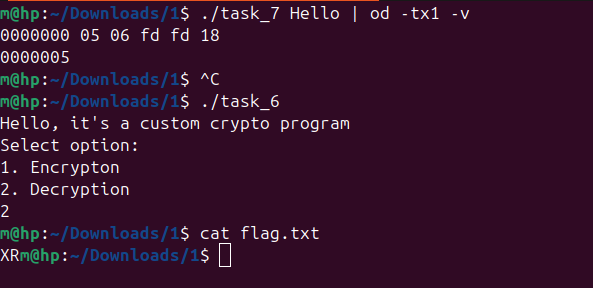
\includegraphics[width=1\linewidth]{static/_task_7}

Также я так и не нашел зависимость task\_2 от task\_7
